\appendix
\section*{Appendix}


\section{Implementation details.}
\label{section:impl_details}

In this section, we provide implementation details for our algorithm.
\Cref{alg:conparison} provides a side-by-side comparison of SDS and our algorithm. 

\begin{figure}[h!]
    \centering
    \begin{minipage}{.5\textwidth}
        \centering
        \begin{algorithm}[H]
            \caption{Dreamfusion (SDS)}\label{alg:original_dreamfusion}
            \begin{algorithmic}\footnotesize
                \Require
                    $\psi \in \mathbb{R}^N$ {- parametrized 3D shape} \\
                    $\mathcal{C}$ {- set of cameras around the 3D shape} \\
                    $y$ {- text prompt} \\
                    $g: \mathbb{R}^N \times \mathcal{C} \rightarrow \mathbb{R}^{n \times n}$ {- differentiable renderer} \\
                    $\epsilon_\theta^{(t)} : \mathbb{R}^{n \times n} \rightarrow \mathbb{R}^{n \times n}$ {- trained diffusion model}
                \Ensure {3D shape} $\psi$ {of} $y$

                \Procedure{Dreamfusion}{$y$}
                \For{$i$ in range($n\_iters$)}
                    \State \textcolor{Red}{$t  \gets \text{Uniform}(0, 1)$}  
                    % \State $t  \gets \text{Uniform}(0, 1)$  
                    \State $c \gets \text{Uniform}(\mathcal{C})$    
                    \State \textcolor{Red}{$\epsilon \gets \text{Normal}(0, I)$ }  
                    % \State $\epsilon \gets \text{Normal}(0, I)$
                    \State $x_t \gets \sqrt{\alpha(t)} g(\psi, c) + \sqrt{1 - \alpha(t)}\epsilon$   
                    \State $\nabla_\psi\mathcal{L}_{SDS} = \sigma(t) \left[\epsilon_\theta^{(t)}\left(x_t, y\right)  - \epsilon \right] \frac{\partial g}{\partial \psi}$   
                    \State $\text{Backpropagate } \nabla_\psi\mathcal{L}_{SDS}$
                    \State $\text{SGD update on } \psi$
                \EndFor
                \EndProcedure
            \end{algorithmic}
        \end{algorithm}
    \end{minipage}%
    \begin{minipage}{.5\textwidth}
        \centering
        \begin{algorithm}[H]
            \caption{Ours (\ourmethod)}\label{alg:suggested_algorithm}
            \begin{algorithmic}\footnotesize
                \Require
                    $\psi \in \mathbb{R}^N$ {- parametrized 3D shape} \\
                    $\mathcal{C}$ {- set of cameras around the 3D shape} \\
                    $y$ {- text prompt} \\
                    $g: \mathbb{R}^N \times \mathcal{C} \rightarrow \mathbb{R}^{n \times n}$ {- differentiable renderer} \\
                    $\epsilon_\theta^{(t)} : \mathbb{R}^{n \times n} \rightarrow \mathbb{R}^{n \times n}$ {- trained diffusion model}
                \Ensure {3D shape} $\psi$ {of} $y$

                \Procedure{Ours}{$y$}
                \For{$i$ in range($n\_iters$)}
                    \State \textcolor{Green}{$t  \gets 1 - i / n\_iters$}   
                    \State $c \gets \text{Uniform}(\mathcal{C})$   
                    \State \textcolor{Green}{$\epsilon \gets \kappa^{t + \tau}_y(g(\psi, c))$} %+ \eta\sqrt{1 - \alpha(t)}\mathcal{N}(0, I)   
                    \State $x_t \gets \sqrt{\alpha(t)} g(\psi, c) + \sqrt{1 - \alpha(t)}\epsilon$ 
                    \State $\nabla_\psi\mathcal{L}_{SDS} = \sigma(t) \left[\epsilon_\theta^{(t)}\left(x_t, y\right)  - \epsilon \right] \frac{\partial g}{\partial \psi}$   
                    \State $\text{Backpropagate } \nabla_\psi\mathcal{L}_{SDS}$
                    \State $\text{SGD update on } \psi$
                \EndFor
                \EndProcedure
            \end{algorithmic}
        \end{algorithm}
    \end{minipage}
    \caption{
        Comparison of the original SDS algorithm and our proposed changes.
    }
    \label{alg:conparison}
\end{figure}

Our implementation uses the following choice of $\kappa^t_y$:
\begin{equation}
    \begin{split}
    H(t) &= 0.3 \sqrt{1  - \alpha(t)} \epsilon_{H} \text{~, where~} \epsilon_{H} \sim \mathcal{N}(0, I)\\
        \kappa^{t}_y(x) &= \textrm{ddim\_inversion}(x, t) + H(t)
    \end{split}
    \label{eq:our_kappa}
\end{equation}

\subsection{Timesteps.}
In \cref{eq:exact_update_kappa}, the added noise inverts \cref{eq:fixed_eq_eps} up to noise level $t$, but the denoising step happens to slightly lower time $t - \tau$ ($t_1$ and $t_2$ in \cref{fig:evolution}, right).
Intuitively, $\tau$ controls the effective step size of the denoising (or image improvement) process.
To accommodate this, we maintain a global time variable $t$ that linearly decays for all the views.
Then, on each update step we run DDIM inversion up to $t + \tau$, where $\tau$ is a small constant.
In practice, we did not find the algorithm to be sensitive to this constant and sample $\tau\sim U(0, \frac{1}{30})$, where $\frac{1}{30}$ is a typical step size in DDIM.


\subsection{Geometry regularization.}
The \emph{Janus problem} is a common issue reported across multiple score distillation works~\cite{poole2022dreamfusion, wang2024prolificdreamer, katzir2023noise}, wherein the model produces frontal views all around the shape due to a bias for views dominant in the training data.
SDS~\cite{poole2022dreamfusion} tackles this problem by augmenting the prompts with information about the view direction.
Our method's variance reduction, however, enabled the use of lower CFG values $\gamma=7.5$ (instead of $100$ for SDS), and as shown in \cref{fig:cfg_effect}, with smaller CFG values, the diffusion model tends to ignore certain parts of the prompts (like ``colored'' for $\gamma < 10$ in \cref{fig:cfg_effect}). 
%
Thus in our algorithm we observe the diffusion model to be less attentive to the prompt augmentation yielding a stronger Janus problem compared to SDS; we also see the same behavior for other baselines that reduce CFG. 
%
To address this issue, we use Perp-Neg~\cite{armandpour2023re} and add a small entropy term $\sim\mathcal N(0, 0.3\sqrt{1 - \alpha(t)}I)$ (\cref{eq:our_kappa}) to the inverted noise to reduce mode-seeking behavior as in~\cite{wang2023taming}.

Another common issue in Score Distillation is the \emph{hollow face illusion}~\cite{hill2007hollow}, which is a tendency to create holes in the geometry of a visually convex shape.
To address this problem, we use a normal map extracted from the volume as described in~\cite{poole2022dreamfusion} and downscaled to $8\times8$ resolution so that only low frequencies are penalized. 
Then, we calculate the sine between adjacent normals (from left to right and top to bottom) and penalize it to be negative.
We activate this loss for the first $40\%$ of the training steps with weight $\alpha_{\text{convexity}}=0.1$ to break the symmetry.

\Cref{section:failure_cases} demonstrates examples of typical failure cases, including the Janus problem and the hollow face illusion.


\subsection{System details.}
We implement our algorithm in \texttt{threestudio}~\cite{threestudio2023} on top of SDS~\cite{poole2022dreamfusion}.
We use Stable Diffusion 2.1~\cite{Rombach_2022_CVPR} as the diffusion model.
For volumetric representation 
we use InstantNGP~\cite{muller2022instant}.
Instead of randomly sampling time $t$ as in SDS, we maintain a global parameter $t$ that linearly decays from $1$ to $0.2$ (lower time values do not have a significant contribution).
Next, for each step we render a $512\times512$ random view and infer $\kappa^{t + \tau}$ by running DDIM inversion for $\texttt{int}(10t)$ steps---i.e.\ we use 10 steps of DDIM inversion for $t=1$ and linearly decrease it for smaller $t$.
We use NVIDIA A6000 GPUs and run each generation for $10k$ steps with learning rate of $10^{-2}$, which takes approximately 2 wall clock hours per shape generation.

\subsection{Prompts used in the quantitative evaluation}
\begin{verbatim}
    "A car made out of sushi"
    "A delicious croissant"
    "A small saguaro cactus planted in a clay pot"
    "A plate piled high with chocolate chip cookies"
    "A 3D model of an adorable cottage with a thatched roof"
    "A marble bust of a mouse"
    "A ripe strawberry"
    "A rabbit, animated movie character, high detail 3d mode"
    "A stack of pancakes covered in maple syrup"
    "An ice cream sundae"
    "A baby bunny sitting on top of a stack of pancakes"
    "Baby dragon hatching out of a stone egg"
    "An iguana holding a balloon"
    "A blue tulip"
    "A cauldron full of gold coins"
    "Bagel filled with cream cheese and lox"
    "A plush dragon toy"
    "A ceramic lion"
    "Tower Bridge made out of gingerbread and candy"
    "A pomeranian dog"
    "A DSLR photo of Cthulhu"
    "Pumpkin head zombie, skinny, highly detailed, photorealistic"
    "A shell"
    "An astronaut is riding a horse"
    "Robotic bee, high detail"
    "A sea turtle"
    "A tarantula, highly detailed"
    "A DSLR photograph of a hamburger"
    "A DSLR photo of a soccer ball"
    "A DSLR photo of a white fluffy cat" 
    "A DSLR photo of a an old man"
    "Renaissance-style oil painting of a queen"
    "DSLR photograph of a baby racoon holding a hamburger, 80mm"
    "Photograph of a black leather backpack"
    "A DSLR photo of a freshly baked round loaf of sourdough bread"
    "A DSLR photo of a decorated cupcake with sparkling sugar on top"
    "A DSLR photo of a dew-covered peach sitting in soft morning light"
    "A photograph of a policeman"
    "A photograph of a ninja"
    "A photograph of a knight"
    "An astronaut"
    "A photograph of a firefighter"
    "A Viking panda with an axe"
\end{verbatim}

\section{Comparison with Interval Score Matching}
\label{sec:ism_comparison}
In this section, we extensively compare our algorithm with Interval Score Matching (ISM)~\cite{liang2023luciddreamer}.

\paragraph{Theoretical assumptions.}
ISM empirically observes that ``pseudo-GT’’ images used to guide Score Distillation Sampling (SDS) are sensitive to their input and that the single-step generation of pseudo-GT yields over-smoothing.
From these observations, starting with SDS guidance, ISM adds DDIM inversion and multi-step generation to empirically improve the stability of the guidance.
In contrast, our work starts with 2D diffusion sampling to re-derive score-distillation guidance and motivate improvements.
That is, our work formally connects SDS to well-justified techniques in 2D sampling.

\paragraph{DDIM inversion.}
In ISM, the empirically motivated DDIM inversion is at the basis of the derivation of the final update rule.
We suggest a general form of the noise term \cref{eq:fixed_eq_eps}, for which \textit{DDIM inversion is just one possible solution}.
Our theoretical insights are agnostic to particular algorithms of root-finding, which makes it possible to use more efficient solutions in future research (e.g.\ train diffusion models as invertible maps to sample noise faster).

\paragraph{Guidance term.}
The update rules provided in our \cref{eq:exact_update_kappa} and ISM’s eq.17 have two main differences:

\begin{enumerate}
    \item \textbf{Full vs.\ interval noise.}
    Assuming DDIM inversion finds a perfect root of our stationary equation, ISM’s update rule can take a similar form to ours \cref{eq:exact_update_kappa} (interval noise is equal to $\kappa$ if \cref{eq:fixed_eq_eps} is satisfied).
    However, as shown in \cref{fig:kappa_ablation}, DDIM inversion does not find a perfect root, and thus the two forms are not equivalent.
    Our theory shows that the full noise term is more accurate.
    We also show the effect of choosing one term vs.\ another in \cref{fig:ablation_with_ism}.

    \item \textbf{Conditional vs.\ unconditional inversion.}
    Our derivation hints that the roots of \cref{eq:fixed_eq_eps} are prompt-dependent, motivating our use of conditional DDIM inversion (not used in ISM).
    Our \cref{fig:cfg_inversion_3d} shows how unconditional inversion yields over-saturation.
\end{enumerate}

\begin{figure}[h!]
    \centering
    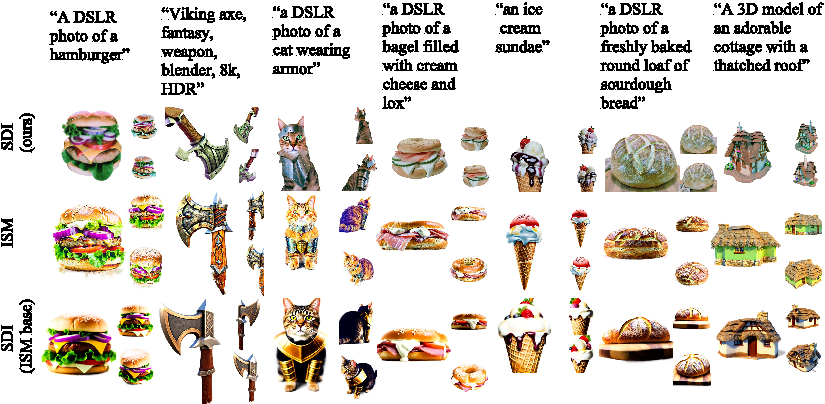
\includegraphics[width=1.\linewidth]{figs/appendix/comparison_with_ism.pdf}
    \vspace{-.1in}
    \caption{
        Comparison of SDI (ours, top) ISM (middle), and SDI in ISM’s code base (ours, bottom).
        To eliminate factors such as 3D representation and initialization, we re-implement our algorithm in the official codebase of ISM.
        See \cref{fig:ablation_with_ism} for the effect of each change made.
    }
    \label{fig:comparison_with_ism}
\end{figure}

\paragraph{Practical Results.}
To control for different design choices (Gaussian Splattings in ISM vs.\ NeRF in ours, etc.) we re-implemented our algorithm in the code base of ISM with only the minimal changes discussed in the previous section.

\begin{figure}[ht]
    \centering
    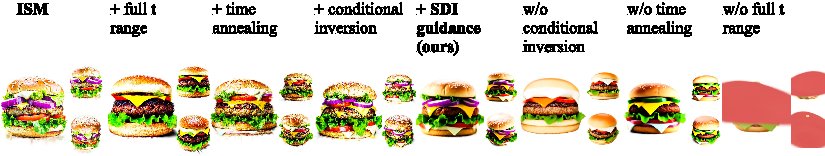
\includegraphics[width=1.\linewidth]{figs/appendix/ablation_with_ism.pdf}
    \vspace{-.1in}
    \caption{
        Ablation of changes made to the code base of Interval Score Matching (ISM).
        Prompt ''A DSLR photo of a hamburger``.
        We start with the official implementation of ISM and add only four changes to match ours (all the hyper-parameters remain tuned for ISM): 
            1. instead of sampling t from U(0.02, 0.5) we sample it from U(0.1, 0.98); 
            2. introduce linear time annealing; 
            3. use conditional DDIM inversion with negative guidance; 
            4. use SDI guidance, i.e.\ second term in the guidance difference is the full noise added to
    }
    \label{fig:ablation_with_ism}
\end{figure}

\Cref{fig:comparison_with_ism} provides a qualitative comparison using the prompts and settings in ISM’s code.
\Cref{fig:ablation_with_ism} shows the effect of each change made to ISM guidance.
\Cref{tab:comparison_with_ism} the quantitative comparison (ISM code base for both).

\begin{table}[ht]
\caption{
        Quantitative comparisons between SDI (ours) and ISM.
    }
    \centering
    \begin{adjustbox}{width=\linewidth}
        \begin{tabular}{@{}lccccccc@{}}
            \hline
            Method & CLIP Score ($\uparrow$) & \multicolumn{3}{c}{CLIP IQA (\%, $\uparrow$)} & ImageReward ($\uparrow$) & Time & VRAM \\ \cmidrule(l){3-5}
                   &                         & ``quality'' & ``sharpness'' & ``real''       &                          &      &      \\ \midrule 
            ISM, 5k steps & \textbf{28.60±2.03} & 0.85±0.02 & 0.98±0.01 & 0.98±0.01 & -0.52±0.48 & 45min & 15.4GB \\
            SDI (ours), 5k steps & 28.47±1.29 & \textbf{0.88±0.03} & \textbf{0.99±0.00} & 0.98±0.01 & \textbf{-0.30±0.32} & 43min & 15.4GB \\
            \hline
        \end{tabular}
    \end{adjustbox}
    \label{tab:comparison_with_ism}
\end{table}

% \begin{table}[h]
% \centering
% \caption{
%     Quantitative comparisons to baselines for text-to-3D generation, evaluated by CLIP Score and CLIP IQA.
%     We report mean and standard deviation across 43 prompts and 50 views for each.\vspace{-.15in}
% }
% \label{tab:comparison}
% \
% \begin{adjustbox}{width=\linewidth}

% \begin{tabular}{@{}lccccccc@{}}
%     \toprule
%     Method                          & CLIP Score ($\uparrow$) & \multicolumn{3}{c}{CLIP IQA (\%) $\uparrow$} & Diverged (\%) $\downarrow$& Time & VRAM \\ \cmidrule(l){3-5}
%                                     &                         & ``quality'' & ``sharpness'' & ``real''       & & &  \\ \midrule 
%     SDS \cite{poole2022dreamfusion}, $10k$ steps         & $29.81 \pm 2.49$ & $76 \pm 6.6$  & $99 \pm 1.2$ & $98 \pm 2.4$ & $18.6$ & 66min & 6.2GB\\
%     SJC \cite{wang2023score},  $10k$ steps               & $30.39 \pm 1.98$ & $76 \pm 6.4$  & $99 \pm 0.1$ & $98 \pm 1.1$ & $11.6$ & 13min & 13.1GB\\
%     VSD \cite{wang2024prolificdreamer}, $25k$ steps      & $33.31 \pm 2.39$ & $77 \pm 6.7$  & $98 \pm 1.3$ & $96 \pm 4.4$ & $23.2$ & 334min & 47.9GB \\
%     ESD \cite{wang2023taming}, $25k$ steps               & $32.79 \pm 2.15$ & $77 \pm 7.2$  & $98 \pm 1.2$ & $97 \pm 2.7$ & $14.0$ & 331min & 46.8GB\\
%     % ISM (NeRF) \cite{liang2023luciddreamer}, $10k$ steps & $32.79 \pm 2.15$ & $77 \pm 7.2$  & $98 \pm 1.2$ & $97 \pm 2.7$ & $14.0$ & 331min & 46.8GB\\
%     HIFA \cite{zhu2023hifa}, $25k$ steps                 & $32.80 \pm 2.35$ & $81 \pm 6.5$  & $98 \pm 1.5$ & $97 \pm 1.2$ & $4.7$ & 235min & 46.4GB \\
%     \textbf{\ourmethod(ours), $10k$ steps}                           & $33.47 \pm 2.49$ & $82 \pm 6.3$  & $98 \pm 1.3$ & $97 \pm 1.2$ & $4.7$ & 119min & 39.2GB\\
%     \bottomrule
%     \vspace{-.15in}
% \end{tabular}
% \end{adjustbox}
% \end{table}



\paragraph{Summary.}
We bridge the gap between experimentally-based score distillation techniques and theoretically-justified 2D sampling.
Both SDS and ISM can be seen as different approaches to finding roots of \cref{eq:fixed_eq_eps}.
This theoretical insight allows us to modify both ISM and SDS, reducing over-saturation for the first and improving general quality of the second. 

% \vspace{-5pt}
\section{Diversity of the generations}
\label{sec:diversity}
Next, we explore the diversity of the results generated by our method.
\Cref{fig:results_diversity} depicts generated shapes for different seeds and prompts. 
Generations with our method exhibit a certain degree of diversity in local details, but are mostly the same at a coarse level.
This is similar to the reported results in other works on score distillation \cite{poole2022dreamfusion, wang2024prolificdreamer}.
We plan to address this problem in future research.

\begin{figure}[h]
    \centering
    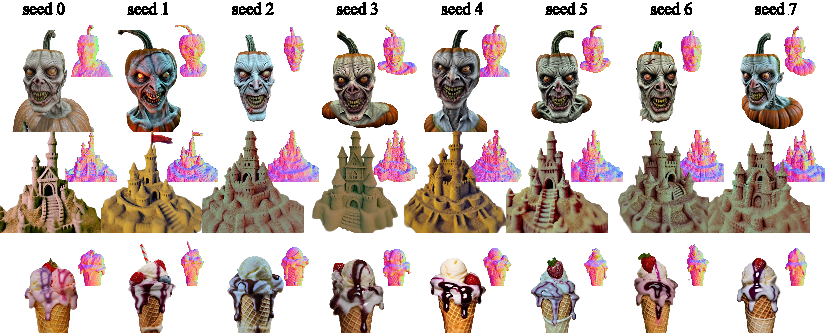
\includegraphics[width=1.\linewidth]{figs/appendix/results_diversity_ablation.pdf}
    \vspace{-.1in}
    \caption{
        Examples of generations with SDI (ours) for different seed values.
        Prompts are ``Pumpkin head zombie, skinny, highly detailed, photorealistic'' (top row),
            ``A highly-detailed sandcastle'' (middle row),
            ``An ice cream sundae'' (bottom row).
    }
    \label{fig:results_diversity}
\end{figure}

\clearpage

Additionally, we noticed a minimal diversity in human generations.
For example, \cref{fig:same_face} demonstrates generated shapes for 3 prompts related to different professions. 

\begin{figure}[h]
    \centering
    \vspace{-.2in}
    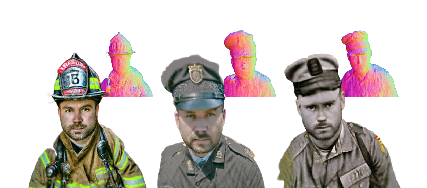
\includegraphics[width=0.5\linewidth]{figs/appendix/limited_diversity_results.pdf}
    \vspace{-.07in}
    \caption{
        Examples of limited diversity across different human-related prompts: 
        ``a photo of a firefighter'', ``a photo of a policeman'', ``a photo of a soldier.''
    }
    \label{fig:same_face}
\vspace{-10pt}
\end{figure}

\section{Visual comparison of noise patterns}
\label{sec:inferred_noises}

\begin{figure}[b!]
    \centering
    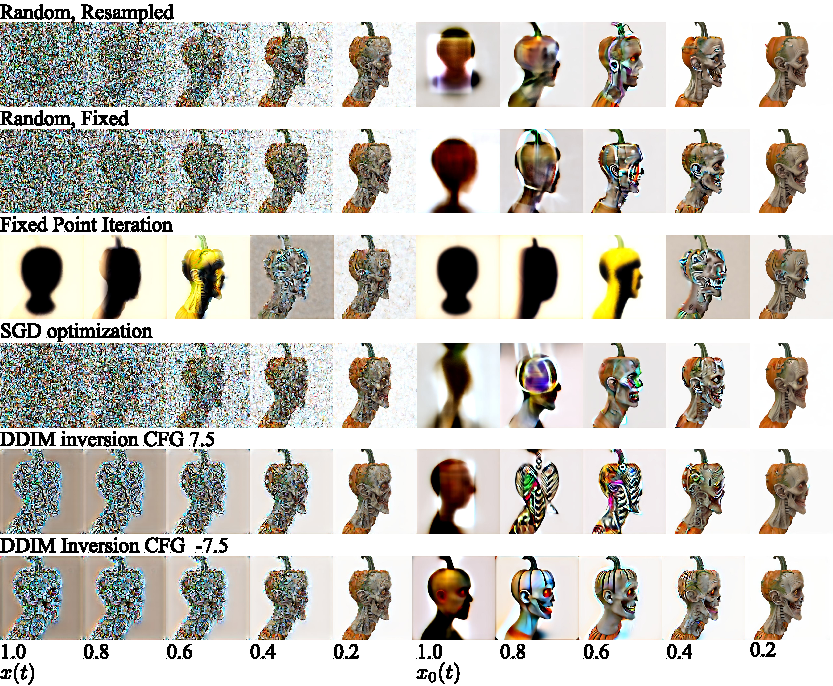
\includegraphics[width=1.\linewidth]{figs/kappa_ablation_noise_copmarison.pdf}
    \vspace{-.1in}
    \caption{
        Examples of noisy images (left part) obtained for different choices of $\kappa_y^t$.
        On the right part, a single step denoised images are presented for the corresponding noisy images.
    }
    \label{fig:kappa_ablation_noise_samples}
\end{figure}


In this section, we provide additional examples of the noise samples obtained with different $\kappa_y^t$. 
As can be seen from \cref{fig:kappa_ablation_noise_samples}, optimization with SGD almost does not change the noise pattern compared to random sampling. 
Fixed-point iterations drift in a notable but counterproductive direction, and the single-step prediction from the obtained noisy images (depicted on the right side) degrades. 
DDIM inversion with $\gamma_{\text{inv}}=7.5$ and $\gamma_{\text{inv}}=-7.5$ produces similar noise patterns located around the ``meaningful'' parts of the image; however, $\gamma_{\text{inv}}=-7.5$ results in noise patterns that are much more compatible with the single-step denoising procedure used in SDS, leading to much more accurate details appearing for earlier $t$.

\section{CFG for inversion in 2D}
\label{sec:cfg_inv_ablation_apendix}
In this section, we provide additional experiments testing the DDIM inversion strategy and study the performance of different combinations of the CFG value on the inversion stage ($\gamma_{\text{inv}}$) and on the forward pass ($\gamma_{\text{fwd}}$).
In particular, in \cref{fig:cfg_inversion_2d} we at first generate an image with $30$ steps of DDIM (left-most image) and $\gamma=7.5$.
Then we run DDIM in the opposite direction of $t$ with $\gamma_{\text{inv}}$ all the way to $t=1$.
Finally, we use the obtained noise sample as an initialization for a new DDIM inference with $\gamma_{\text{fwd}}$.
Ideally, the final image will correspond to the input of the inversion algorithm.

\Cref{fig:cfg_inversion_2d} shows that when inverting the DDIM trajectory starting with a clean image, the best inversion strategy uses $\gamma_{\text{inv}} = 0$ and then regenerates the image via DDIM with $\gamma_{\text{fwd}} = 0$.
\cite{miyake2023negative} suggests this approach, which inverts the computation almost perfectly.
Other approaches introduce bias and only approximate  the image on the forward pass.

As we have seen in \cref{sec:cfg_inv_ablation}, in 3D, the story is different: $\gamma_{\text{inv}}=\gamma_{\text{fwd}}=0$ fails to generate any meaningful shape.
We explain this behavior by the fact that in our 2D experiment, the original image contains class information; inverting with $\gamma_{\text{inv}} = 0$ encodes this information into the noise and thus does not need additional CFG during reconstruction.
In 3D generation, however, the initial NeRF does not contain class information and needs bigger CFG on the forward pass.
Additionally, \cref{fig:cfg_inversion_2d} demonstrates the inversion quality of an entire DDIM trajectory, whereas \cref{eq:exact_update_kappa} we are interested in inverting a single-step denoising only. what might explain the fact that seemingly bad inversion quality of $\gamma_{\text{fwd}}=-\gamma_{\text{inv}}=7.5$ yields much better results in 3D.

\begin{figure}[htbp!]
    \centering
    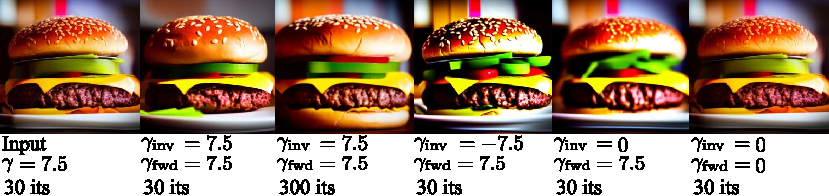
\includegraphics[width=1.\linewidth]{figs/CFG_inversion_ablation_2D.pdf}
    \vspace{-.2in}
    \caption{
        Comparison of different DDIM inversion strategies in 2D.
        Here, we compare the quality of inversion, i.e., the forward pass is the entire DDIM trajectory.
    }
    \label{fig:cfg_inversion_2d}
\end{figure}

\section{ODE derivation}
\label{sec:ode_deriv}
Our derivation in \cref{section:reparametrization} manipulates the time-stepping procedure of DDIM, but a similar argument applies to the ODE version of the method. 
In particular, one can obtain an alternative form of \cref{eq:exact_update_kappa} by reparametrizing the ODE~\cref{eq:DDIM}. 
To do the change of variables in \cref{eq:DDIM} to \cref{eq:x0t} we need to differentiate it with respect to $t$ and evaluate $\frac{d \bar{x}(t)}{dt}$.
Direct differentiation gives us:
\begin{equation}
    \label{eq:dx0t}
     \frac{d x_0(t)}{dt} = \frac{d \bar{x}(t)}{dt} - \epsilon_\theta^{(t)}\left( \frac{ \bar{x}(t)}{\sqrt{\sigma(t)^2 + 1}}, y\right) \frac{d \sigma(t)}{dt} - \sigma(t) \frac{d}{dt} \epsilon_\theta^{(t)} \left( \frac{ \bar{x}(t)}{\sqrt{\sigma(t)^2 + 1}}, y\right).
\end{equation}

Solving for $\frac{d \bar{x}(t)}{dt}$ and merging with \cref{eq:DDIM}, we get:
{\allowdisplaybreaks
\begin{align}
    \epsilon_\theta^{(t)}\left( 
        \frac{ \bar{x}(t)}{\sqrt{\sigma(t)^2 + 1}}, y
    \right) \frac{d \sigma(t)}{dt} 
    &= \frac{d x_0(t)}{dt}
    + \epsilon_\theta^{(t)}\left( 
        \frac{ \bar{x}(t)}{\sqrt{\sigma(t)^2 + 1}}, y
       \right) \frac{d \sigma(t)}{dt} 
    + \sigma(t) \frac{d}{dt} \epsilon_\theta^{t} \left( 
        \frac{ \bar{x}(t)}{\sqrt{\sigma(t)^2 + 1}}, y
      \right)\nonumber
      \\
        \frac{d x_0(t)}{dt} &= -\sigma(t) \frac{d}{dt} \epsilon_\theta^{(t)} \left( \frac{ \bar{x}(t) }{\sqrt{\sigma(t)^2 + 1}}, y\right)\nonumber\\
                            &= -\sigma(t) \frac{d}{dt} \epsilon_\theta^{(t)} \left( \frac{ x_0(t) + \sigma(t)\kappa^t(x_0(t)) }{\sqrt{\sigma(t)^2 + 1}}, y\right)\nonumber\\
                            &= -\frac{d\kappa^t}{dt} (x_0(t)).
\end{align}

Or, expressed in other scaling parameters:
\begin{equation}
    \label{eq:exact_update_kappa_ode}
    \frac{d x_0(t)}{dt} = -\sigma(t) \frac{d}{dt} \epsilon_\theta^{(t)} \left( x_0(t) + \sigma(t)\kappa^t(x_0(t)) , y\right) \text{.}
\end{equation}
}

This expression gives us the DDIM's ODE re-parametrized for the dynamics of $x_0(t)$. 
This ODE is a velocity field that projects a starting image to a conditional distribution learned by the diffusion model.
Discretizing this equation leads to \cref{eq:exact_update_kappa}.


\section{Additional Intuition: Out-of-Distribution Correction}\label{sec:oodview}

Here we provide an intuition why it is so important to regress the noise $\kappa$ instead of randomly sampling it.
In particular, we can look into the data that was used to train $\epsilon_\theta^{(t)}$.
For each $t$, the model has seen only clean images with the corresponding amount of noise $\sigma(t)$.

Consider a noisy or blurry image $\hat{x}_0$.
Our goal is to use our updated ODE to improve it and make it look more realistic.
For $t$ close to $1$, the amount of noise is so big, that for any image $\hat{x}_0$ its noisy version $\hat{x}_0 + \sigma(t)\epsilon$ looks indistinguishable from the training data of the denoiser. This explains why we can successfully use diffusion models to correct out-of-distribution images.

For small $t$, however, the noise levels might be not enough to hide the artifacts of $\hat{x}_0$, so the image becomes out-of-distribution, and the predictions of the model become unreliable. 
We hypothesize, that if instead of randomly sampling $\epsilon$ like in Dreamfusion, we can find such a noise sample, that under the same noise level $t$ the artifacts of $\hat{x}_0$ will be hidden and it will be in-distribution of the denoiser.
This effectively increases the ranges of $t$ where the predictions of the model are reliable and thus improves the generation quality.
This intuition is illustrated in \cref{fig:ood_cones}.

\begin{figure}[h!]
    \centering
    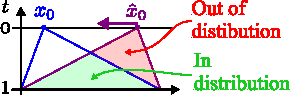
\includegraphics[width=0.5\linewidth]{figs/OOD_intuition.pdf}
    \caption{Schematic for out-of-distribution interpretation.}
    \label{fig:ood_cones}
\end{figure}

\section{Additional Results}

Lastly, we discuss failure cases and showcase additional generations using our methods, along with more baseline comparisons.

\subsection{Failure Cases}
\label{section:failure_cases}
We provide illustrations of typical failure cases of our algorithm in \Cref{fig:contentdrift,fig:hollowface,fig:janus,fig:diffusionanomalies}.

\begin{figure}[hbpt!]
    \centering
    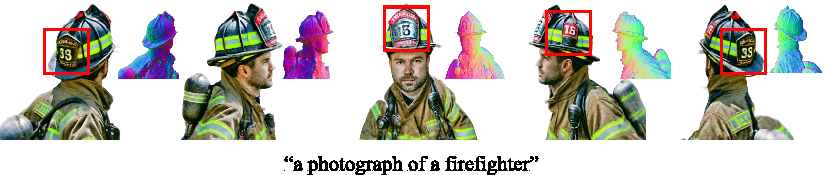
\includegraphics[width=1\linewidth]{figs/appendix/limitation_drift.pdf}
    \vspace{-.2in}
    \caption{\textbf{Content Drift}: due to a limited communication between the frames sometimes we can observe that certain properties ``drift'' around the shape. In this particular example the number on the fireman's hat is different from all the views.\label{fig:contentdrift}}
\end{figure}

\begin{figure}[hbpt!]
    \centering
    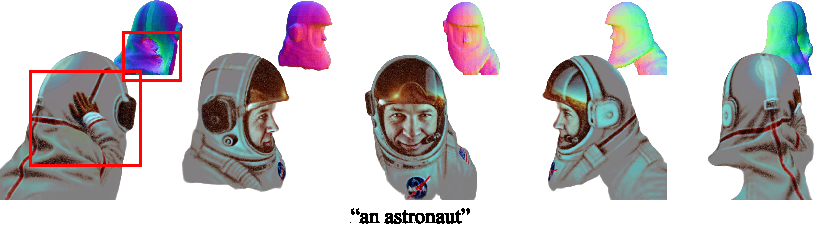
\includegraphics[width=1\linewidth]{figs/appendix/limitation_hollow.pdf}
    \vspace{-.2in}
    \caption{\textbf{Hollow Face Illusion:} some shapes might be generated with a concave hole in the geometry, while the rendering appears to be convex.\label{fig:hollowface}}
    \vspace{-.2in}
\end{figure}

\begin{figure}[hbpt!]
    \centering
    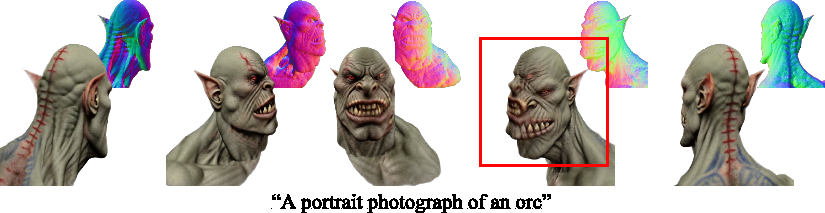
\includegraphics[width=1\linewidth]{figs/appendix/limitation_janus.pdf}
    \vspace{-.2in}
    \caption{\textbf{Janus Problem:} note how the orc has two faces that merge on the second to the right view.\label{fig:janus}}
    \vspace{-.2in}
\end{figure}

\begin{figure}[hbpt!]
    \centering
    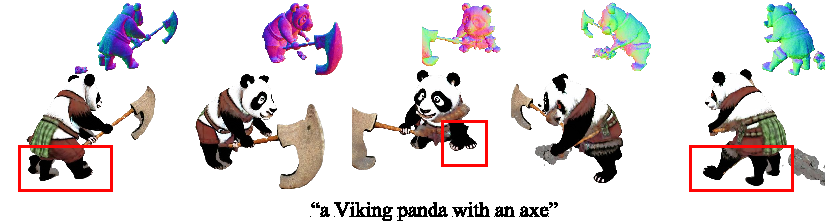
\includegraphics[width=1\linewidth]{figs/appendix/limitation_limbs.pdf}
    \vspace{-.2in}
    \caption{\textbf{Diffusion Anomalies:} performance of our algorithm is limited by the quality of the underlying diffusion model. In this case the generated shape contains a typical failure case of multiple limbs.\label{fig:diffusionanomalies}}
    \vspace{-.2in}
\end{figure}


\subsection{Additional generations}
\label{section:additional_generations}

\Cref{fig:add_res1,fig:add_res2,fig:add_res3,fig:add_res4} provide additional generations produced using our method.

\begin{figure}[hbpt!]
    \centering
    \vspace{-.2in}
    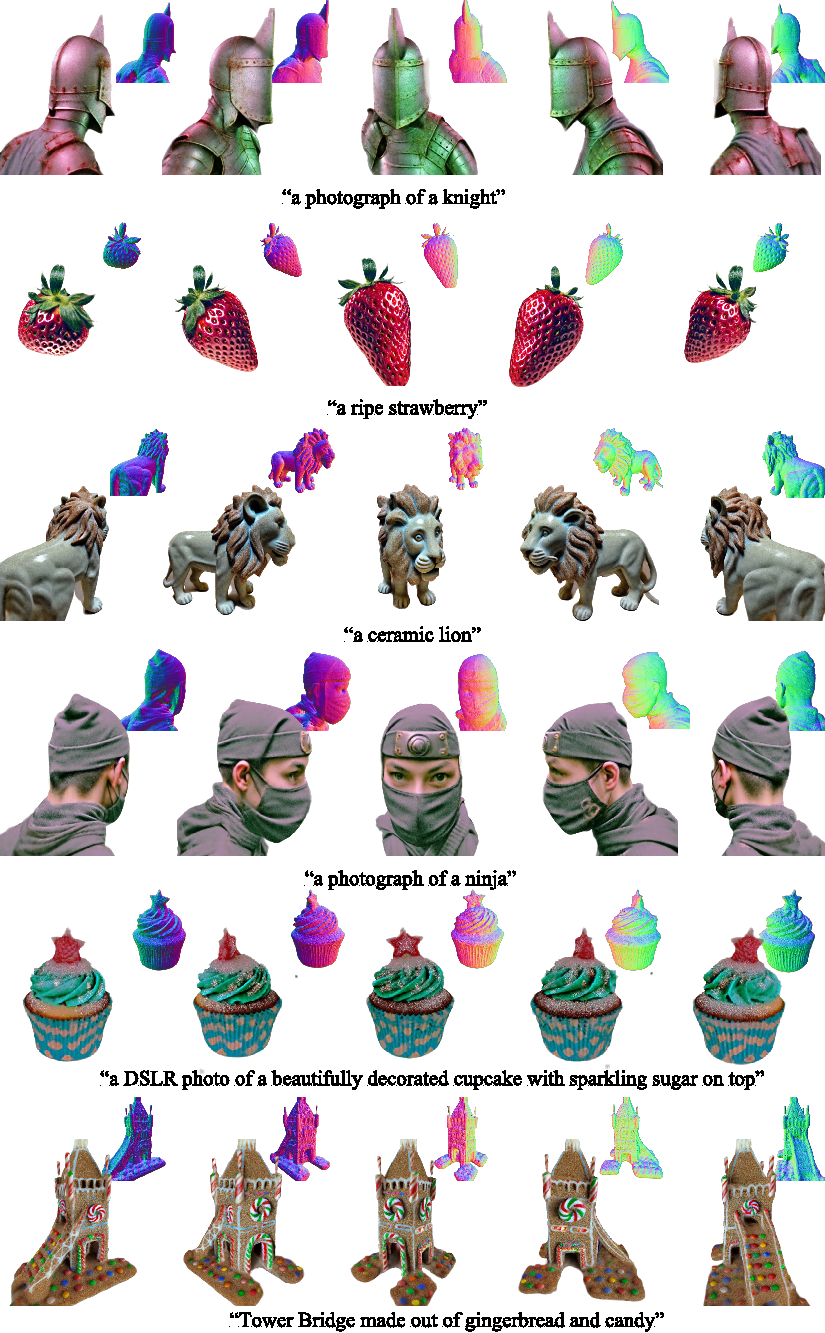
\includegraphics[width=1.\linewidth]{figs/appendix/additional_results_1.pdf}
    \vspace{-.1in}
    \caption{Additional generations from our method.}
    \vspace{-.2in}
    \label{fig:add_res1}
\end{figure}

\begin{figure}
    \centering
    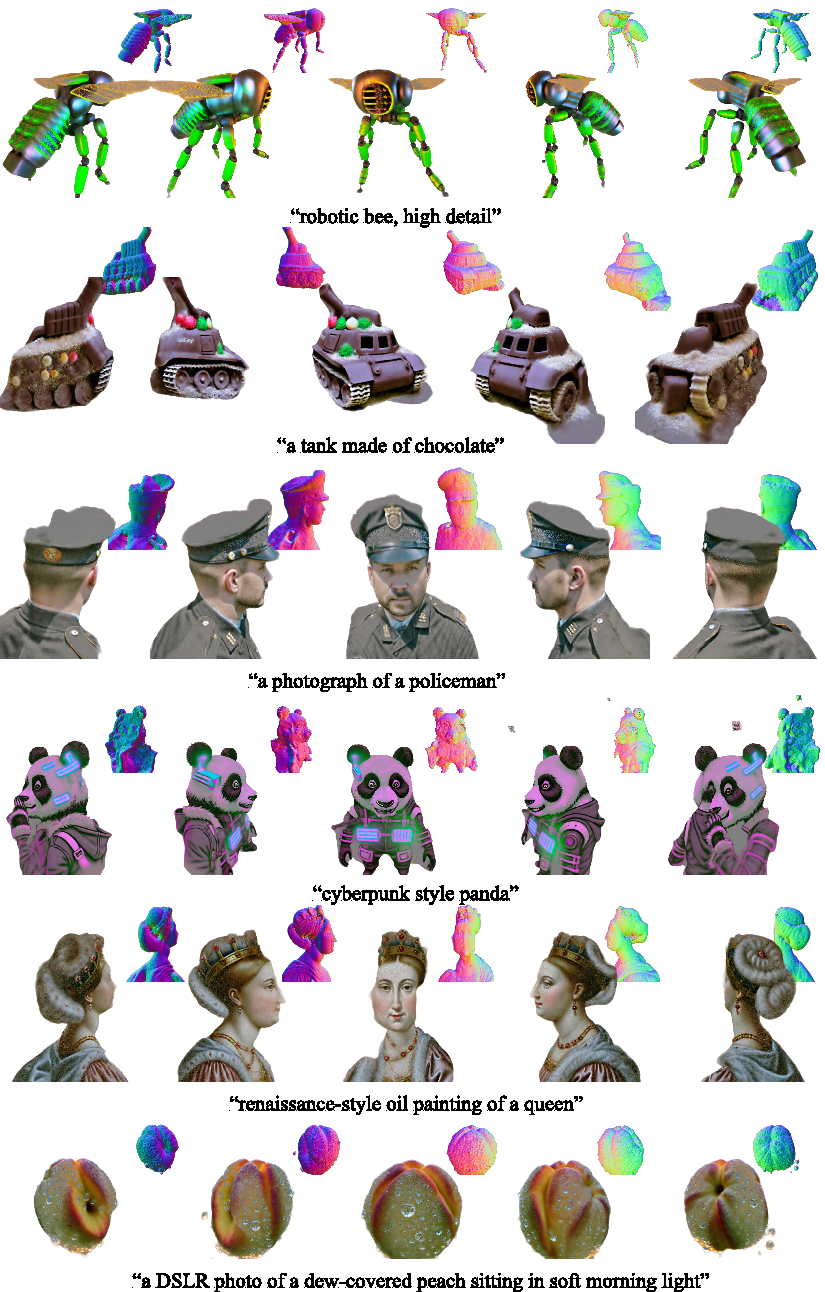
\includegraphics[width=1\linewidth]{figs/appendix/additional_results_2.pdf}
    \vspace{-.1in}
    \caption{Additional generations from our method.}
    \vspace{-.2in}
    \label{fig:add_res2}
\end{figure}

\begin{figure}
    \centering
    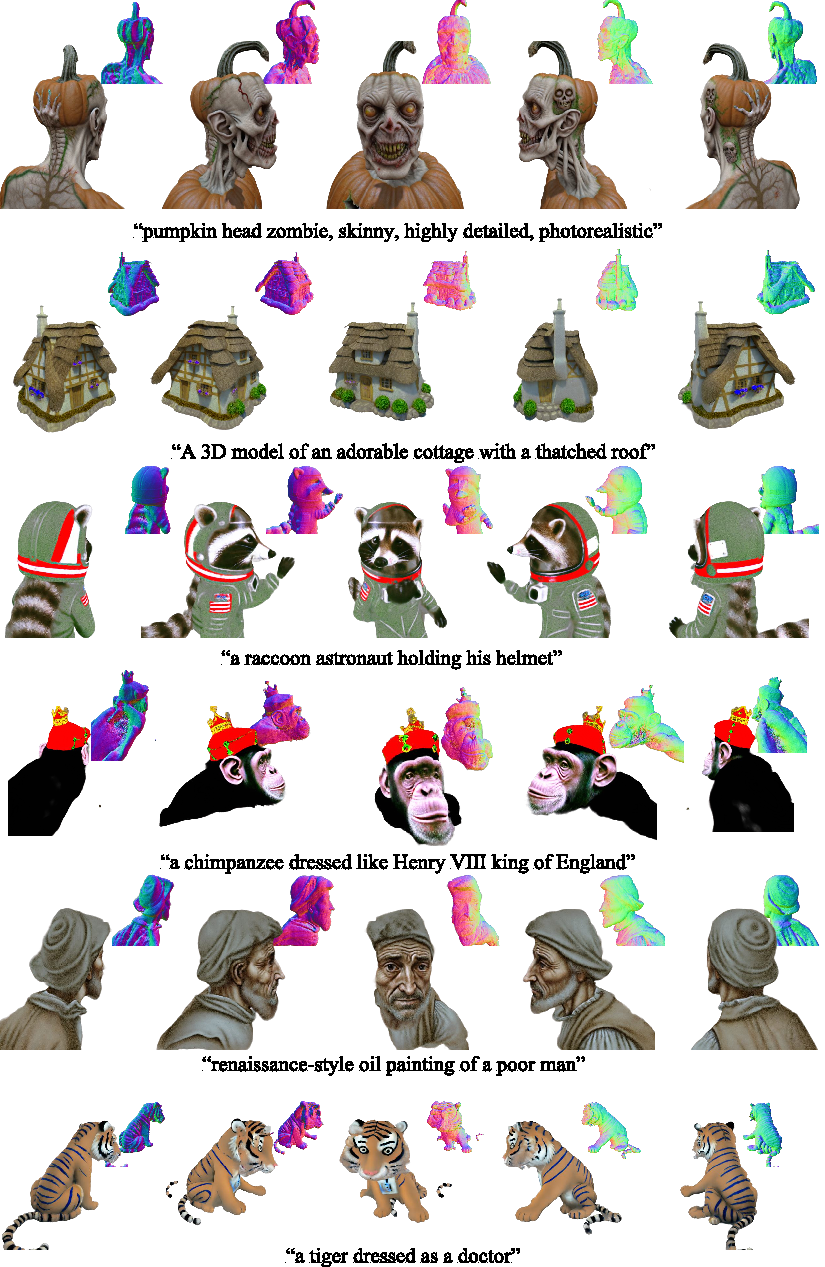
\includegraphics[width=1\linewidth]{figs/appendix/additional_results_3.pdf}
    \vspace{-.1in}
    \caption{Additional generations from our method.}
    \vspace{-.2in}
    \label{fig:add_res3}
\end{figure}

\begin{figure}
    \centering
    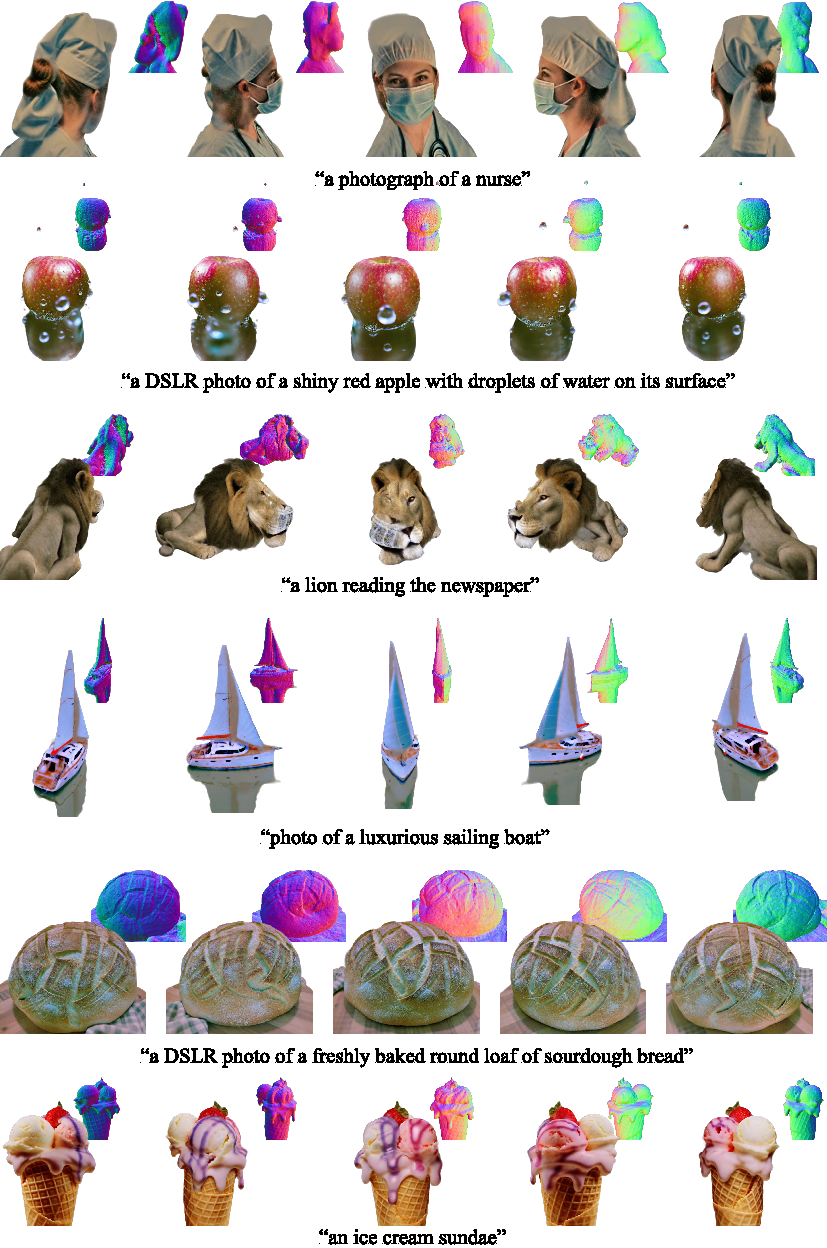
\includegraphics[width=1\linewidth]{figs/appendix/additional_results_4.pdf}
    \vspace{-.1in}
    \caption{Additional generations from our method.}
    \vspace{-.2in}
    \label{fig:add_res4}
\end{figure}



\subsection{Additional comparison with baselines}
\label{sec:additional_comparisons}

We provide additional qualitative comparisons with other score distillation algorithms in \cref{fig:add_comp_compressed1,fig:add_comp_compressed2,fig:add_comp_compressed3}.
We compare with Dreamfusion~\cite{poole2022dreamfusion}, Magic3D~\cite{lin2023magic3d}, Fantasia3D~\cite{chen2023fantasia3d}, Stable Score Distillation (StableSD~\cite{tang2023stable}, Classifier Score Distillation (ClassifierSD~\cite{yu2023text}), Noise-Free Score Distillation (NFSD~\cite{katzir2023noise}), ProlificDreamer or Variational Score Distillation (VSD~\cite{wang2024prolificdreamer}), Interval Score Matching (ISM)~\cite{liang2023luciddreamer}, and HiFA~\cite{zhu2023hifa}.

\begin{figure}
    \centering
    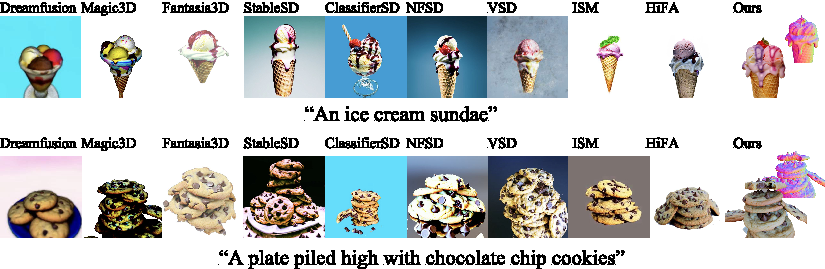
\includegraphics[width=1\linewidth]{figs/appendix/add_comparison_1.pdf}\\
    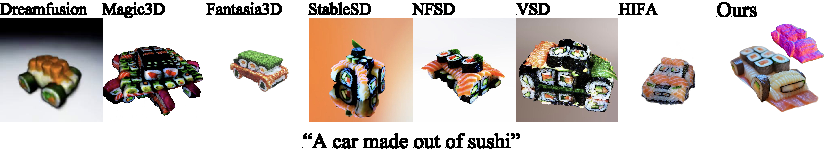
\includegraphics[width=1\linewidth]{figs/appendix/add_comparison_2.pdf}\\
    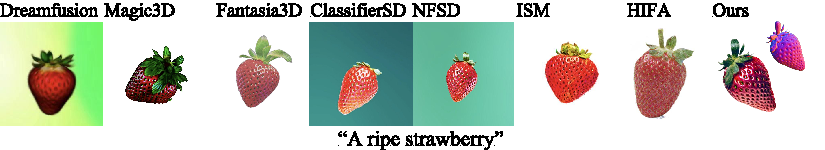
\includegraphics[width=1\linewidth]{figs/appendix/add_comparison_3.pdf}\\
    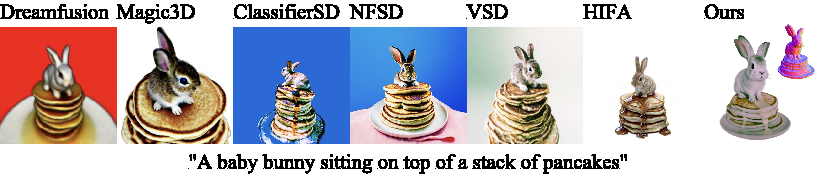
\includegraphics[width=1\linewidth]{figs/appendix/add_comparison_4.pdf}\\
    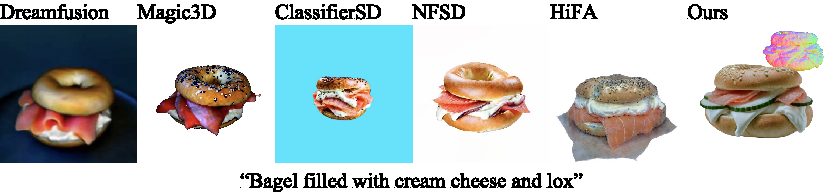
\includegraphics[width=1\linewidth]{figs/appendix/add_comparison_5.pdf}\\
    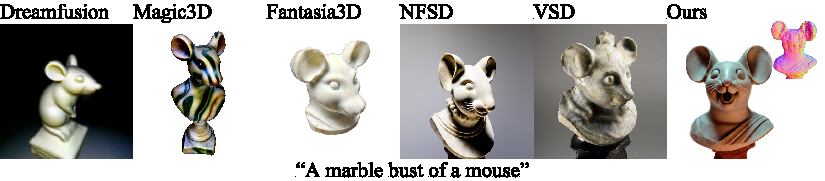
\includegraphics[width=1\linewidth]{figs/appendix/add_comparison_6.pdf}
    \caption{Additional comparisons.}
    \label{fig:add_comp_compressed1}
\end{figure}

\begin{figure}
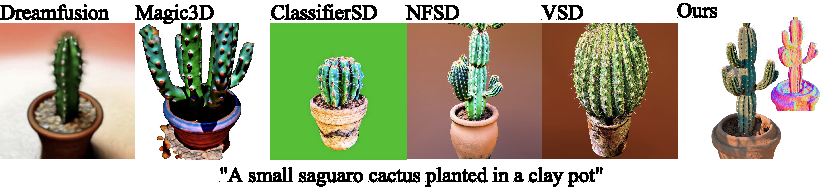
\includegraphics[width=1\linewidth]{figs/appendix/add_comparison_7.pdf}\\
    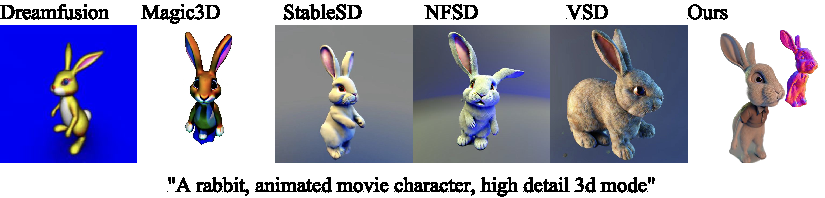
\includegraphics[width=1\linewidth]{figs/appendix/add_comparison_8.pdf}\\
    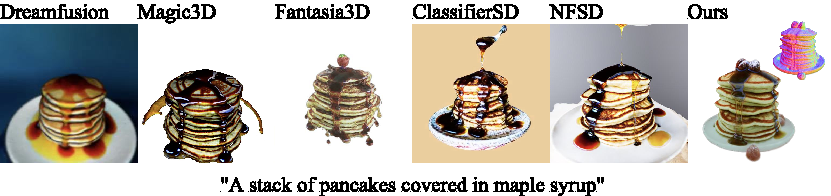
\includegraphics[width=1\linewidth]{figs/appendix/add_comparison_9.pdf}\\
    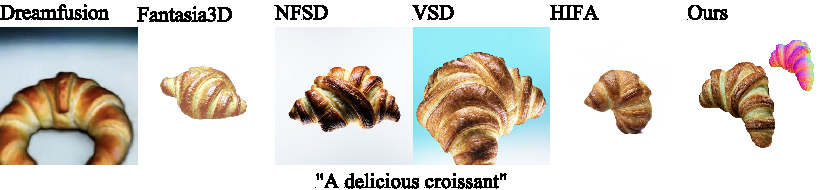
\includegraphics[width=1\linewidth]{figs/appendix/add_comparison_10.pdf}\\
    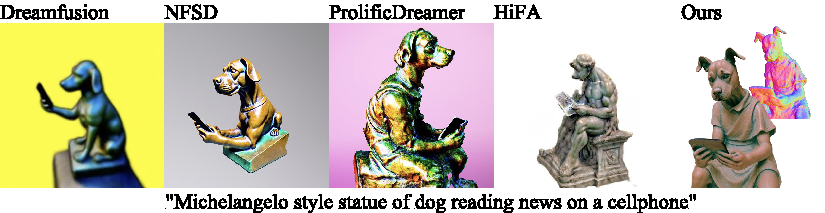
\includegraphics[width=1\linewidth]{figs/appendix/add_comparison_11.pdf}\\
    \caption{Additional comparisons.}
    \label{fig:add_comp_compressed2}
\end{figure}

\begin{figure}
    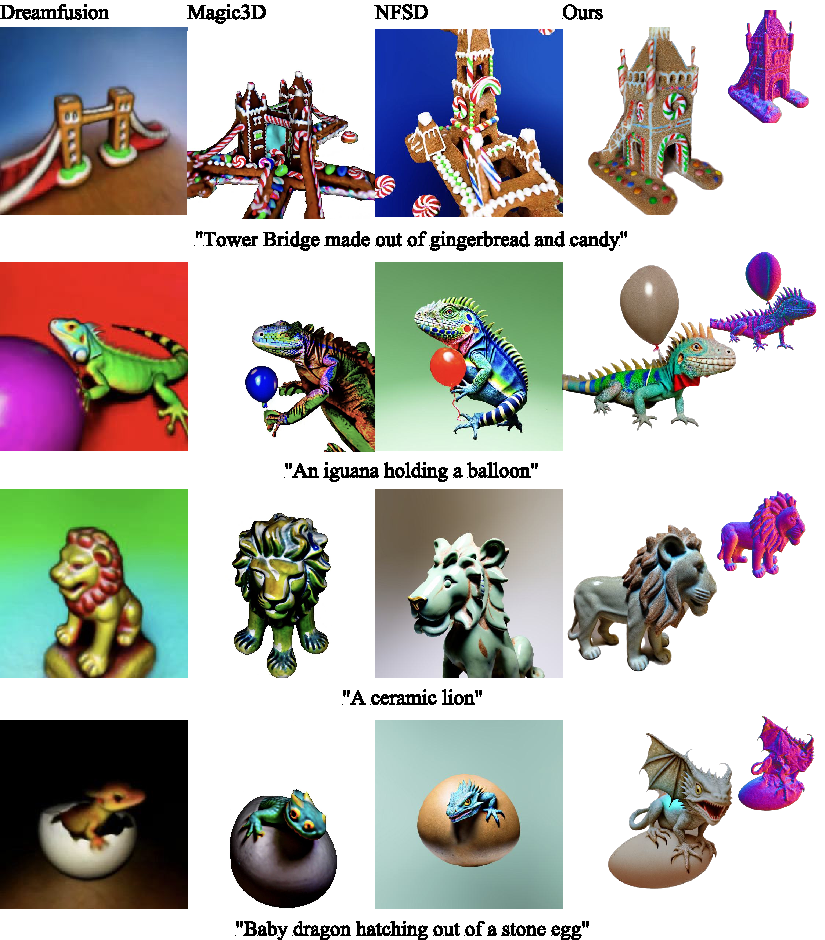
\includegraphics[width=1\linewidth]{figs/appendix/add_comparison_12.pdf}
    \caption{Additional comparisons.}
    \label{fig:add_comp_compressed3}
\end{figure}
